% ============================================================
% Diagrama Entidad-Relacion de la base de datos - App Turismo Comarapa
% Requiere en el preambulo del documento principal:
%   \usepackage{graphicx} % para \includegraphics
%   \usepackage{float}    % para el especificador de posicion [H]
%   \usepackage{array}    % para columnas p{} y el modificador >{\bfseries}
% Imagen asociada: DIAGRAMA_ENTIDAD_RELACION.png / .svg / .pdf (misma carpeta)
% Generado a partir de supabase/ESTRUCTURA_BASE_DE_DATOS.txt y
% supabase/04_SCHEMA_TURISMO_COMARAPA.sql (estado actual, post script 08)
% ============================================================

\subsection*{Diagrama Entidad-Relación}

El modelo de datos reside en el esquema \texttt{public} de una base de
datos \textbf{PostgreSQL} gestionada por Supabase y está compuesto por
\textbf{9 tablas propias} más la tabla \texttt{auth.users}, provista por
Supabase Auth y referenciada desde \texttt{usuarios} mediante una
relación \textbf{1:1} real (llave foránea). La tabla \texttt{categorias}
funciona como catálogo maestro editable por el administrador: cada una
de las seis tablas de contenido turístico (\texttt{lugares},
\texttt{hoteles}, \texttt{restaurantes}, \texttt{gastronomia},
\texttt{actividades} y \texttt{eventos}) se relaciona con ella mediante
\texttt{categoria\_id} (\textbf{1:N}, llave foránea real), y un trigger
(\texttt{fn\_validar\_categoria}) garantiza que la categoría elegida
pertenezca al mismo módulo. La tabla \texttt{restaurantes} se relaciona
además de forma opcional (\textbf{1:N}) con \texttt{gastronomia} a
través de \texttt{restaurante\_id}, indicando dónde encontrar un plato o
bebida típica. Finalmente, \texttt{resenas} implementa una
\textbf{asociación polimórfica}: sus columnas \texttt{entidad} (enum) y
\texttt{entidad\_id} (uuid) apuntan, según el valor de \texttt{entidad},
a una fila de cualquiera de las seis tablas de contenido; esta relación
se dibuja con línea discontinua porque \textbf{no existe una llave
foránea real} en la base de datos (una reseña puede apuntar a distintas
tablas), por lo que la integridad referencial se valida en el código de
la aplicación.

\begin{figure}[H]
\centering
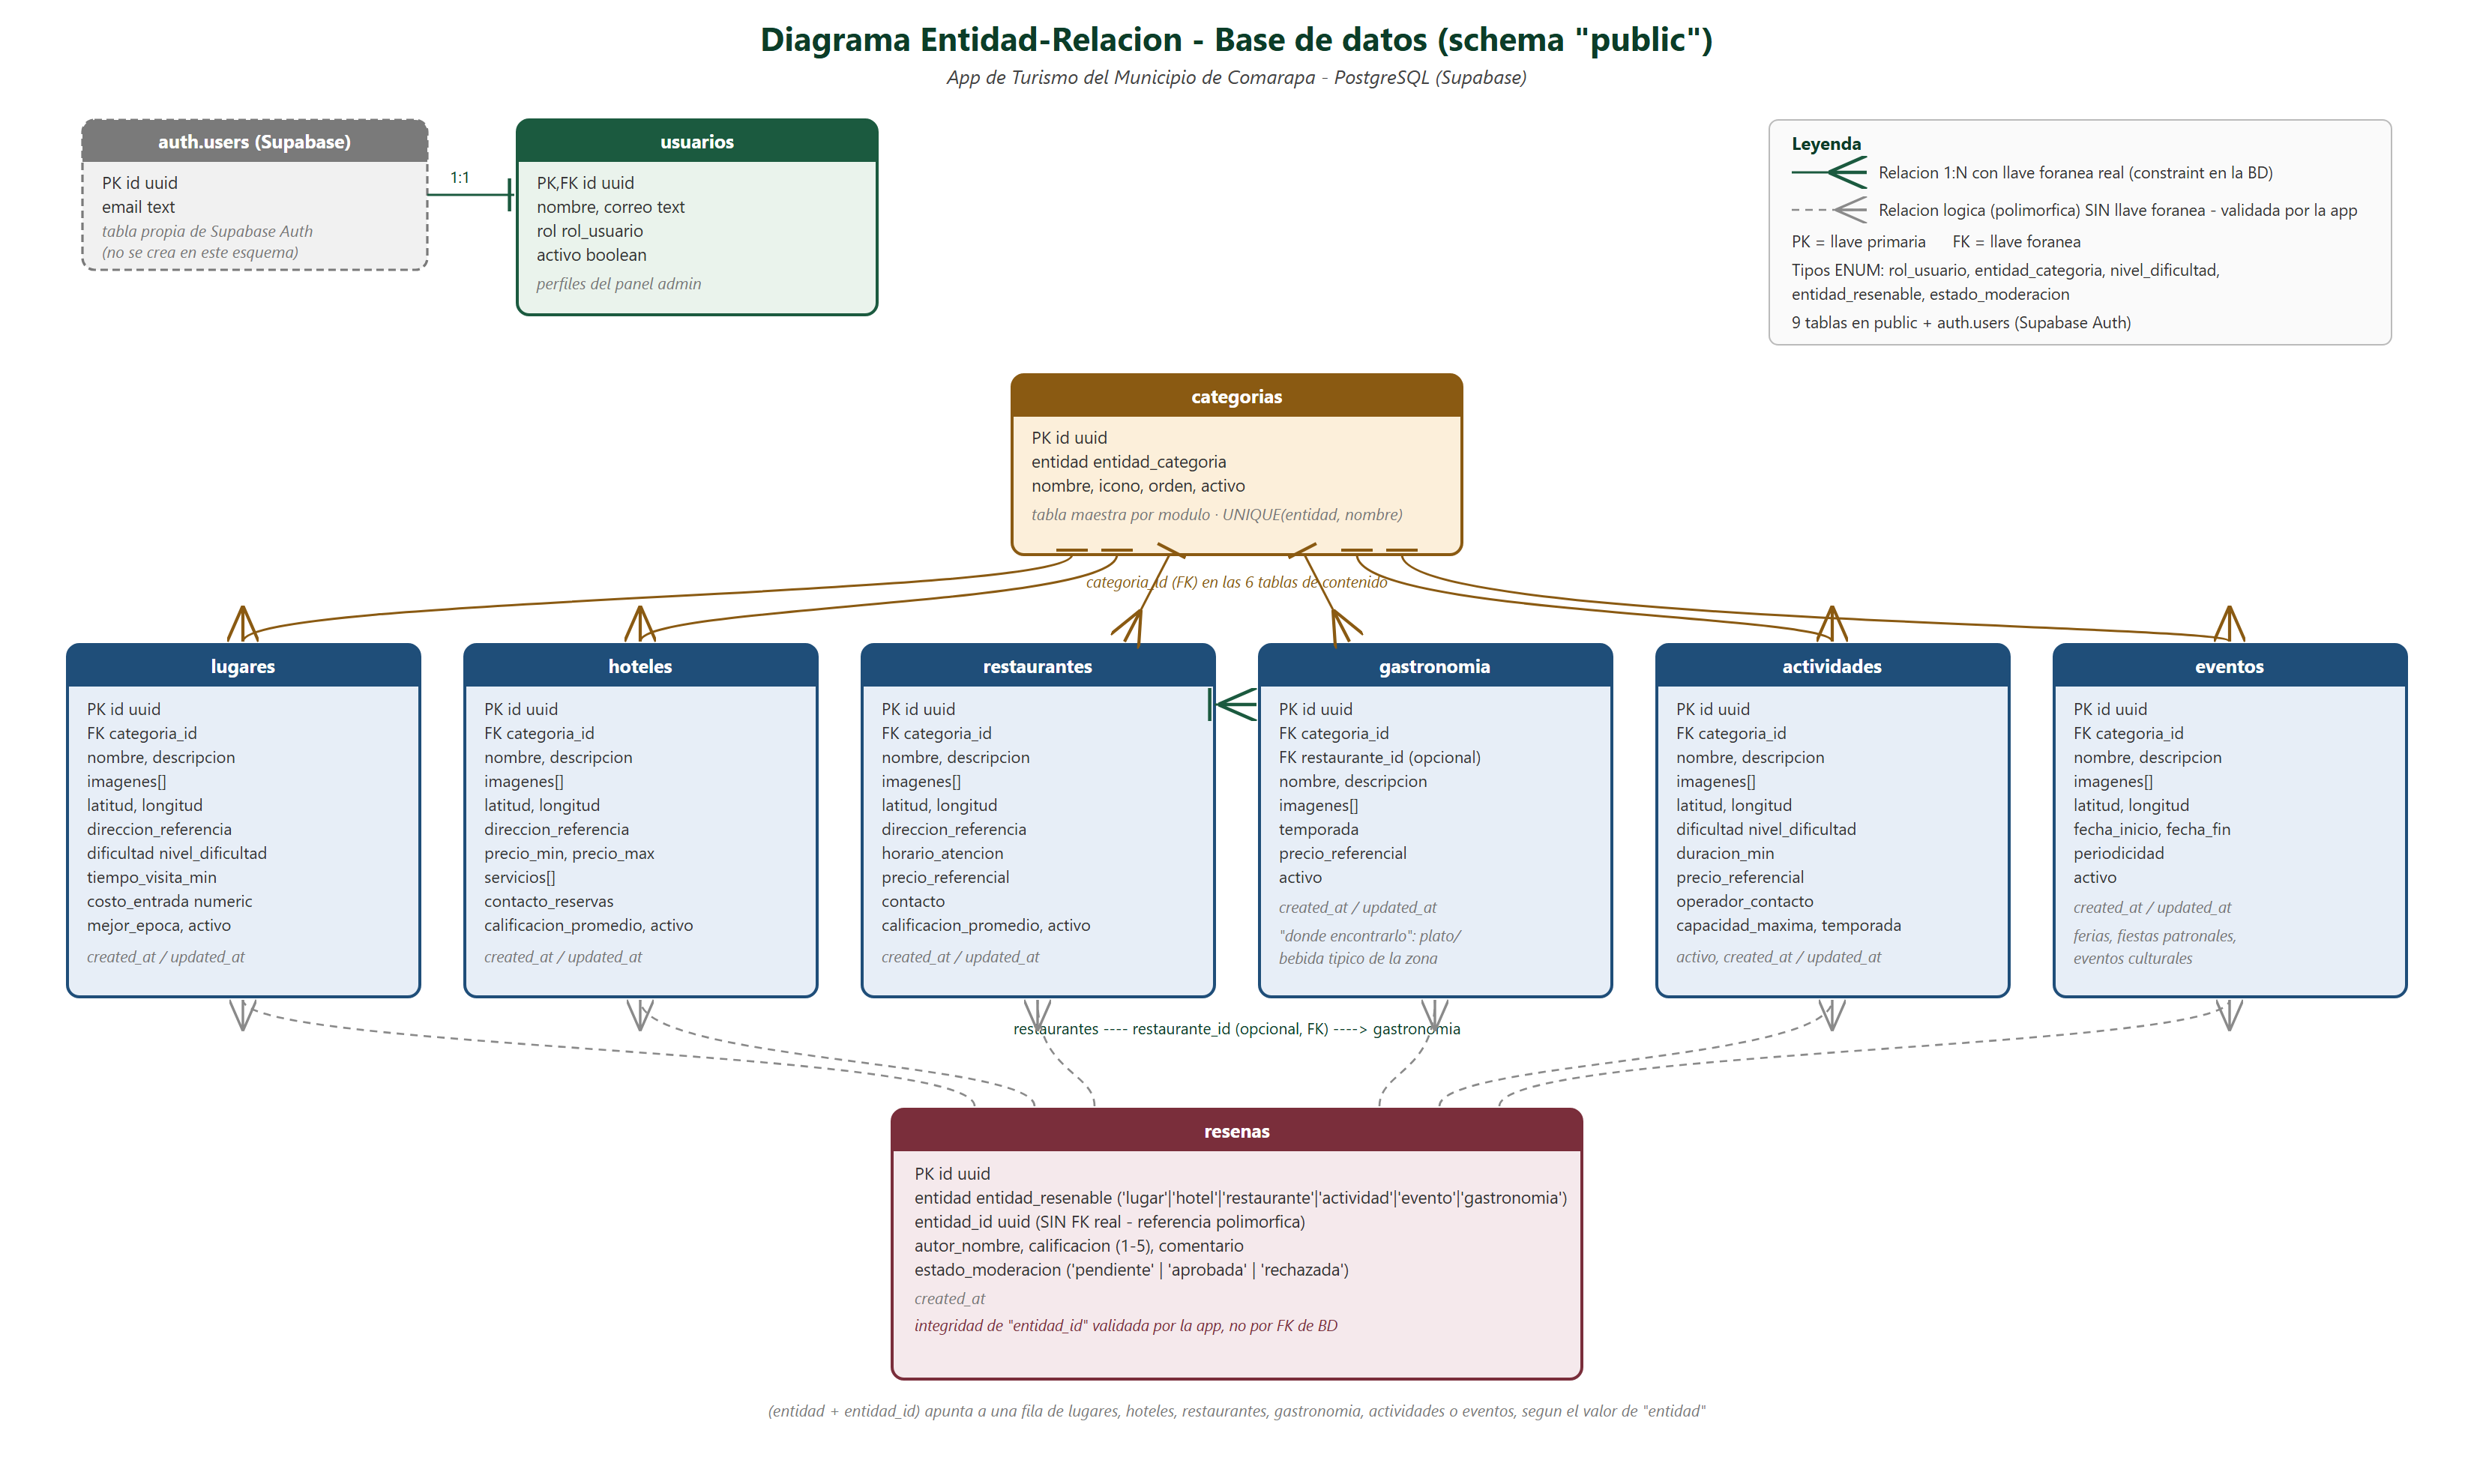
\includegraphics[width=\textwidth]{DIAGRAMA_ENTIDAD_RELACION.png}
\caption{Diagrama entidad-relación de la base de datos de la aplicación de turismo del municipio de Comarapa}
\label{fig:entidad-relacion}
\end{figure}

\begin{table}[H]
\centering
\caption{Resumen de tablas del esquema \texttt{public}}
\label{tab:entidad-relacion}
\renewcommand{\arraystretch}{1.3}
\begin{tabular}{|>{\bfseries}p{2.7cm}|p{5.0cm}|p{5.8cm}|}
\hline
Tabla & Relación principal & Descripción \\ \hline

usuarios & 1:1 con \texttt{auth.users} (FK real) &
Perfiles del panel de administración (rol \texttt{editor} /
\texttt{administrador}). \\ \hline

categorias & Referenciada por las 6 tablas de contenido &
Catálogo de tipos por módulo, editable por el administrador. \\ \hline

lugares & N:1 con \texttt{categorias} &
Lugares turísticos (naturales, arqueológicos, aventura, miradores). \\ \hline

hoteles & N:1 con \texttt{categorias} &
Hospedaje: hoteles, hostales, cabañas, camping. \\ \hline

restaurantes & N:1 con \texttt{categorias}; 1:N (opcional) con \texttt{gastronomia} &
Restaurantes del municipio. \\ \hline

gastronomia & N:1 con \texttt{categorias} y, opcionalmente, con \texttt{restaurantes} &
Platos, bebidas y productos típicos. \\ \hline

actividades & N:1 con \texttt{categorias} &
Actividades turísticas: senderismo, cabalgatas, agroturismo. \\ \hline

eventos & N:1 con \texttt{categorias} &
Eventos y ferias del municipio (ej. Feria del Durazno). \\ \hline

resenas & Relación lógica (polimórfica, sin FK) hacia las 6 tablas de contenido &
Reseñas y calificaciones públicas, sujetas a moderación
(\texttt{pendiente}, \texttt{aprobada}, \texttt{rechazada}). \\ \hline

\end{tabular}
\end{table}

\textit{Nota: las tablas \texttt{municipio}, \texttt{contactos\_emergencia},
\texttt{rutas}, \texttt{rutas\_lugares} y \texttt{rutas\_actividades},
creadas originalmente en el script \texttt{04}, fueron eliminadas de
forma permanente por el script \texttt{08} y ya no existen en la base de
datos; por eso no aparecen en este diagrama.}
